\documentclass{beamer}

\usepackage{fancyvrb}
\usepackage{color, colortbl}
\usepackage{listings}
\usepackage{url}
\usepackage{array}
\usepackage{calc}
\usepackage{ctable}
\usepackage{amsmath}
\usepackage{cite}
\usepackage{graphicx}
\usepackage{listings}
\usepackage{xspace}
\usepackage{hyperref}
\usepackage{subfigure}

\definecolor{lightgray}{rgb}{0.9,0.9,0.9}

\lstset{ %
language=C++,                % choose the language of the code
basicstyle=\tiny,       % the size of the fonts that are used for the code
%numbers=left,                   % where to put the line-numbers
numbers=none,                   % where to put the line-numbers
numberstyle=\scriptsize,      % the size of the fonts that are used for the line-numbers
stepnumber=1,                   % the step between two line-numbers. If it's 1 each line will be numbered
numbersep=15pt,                  % how far the line-numbers are from the code
backgroundcolor=\color{lightgray},  % choose the background color. You must add \usepackage{color}
%backgroundcolor=none,  % choose the background color. You must add \usepackage{color}
showspaces=false,               % show spaces adding particular underscores
showstringspaces=false,         % underline spaces within strings
showtabs=false,                 % show tabs within strings adding particular underscores
frame=single,	                % adds a frame around the code
%frame=none,	                % adds a frame around the code
tabsize=2,	                % sets default tabsize to 2 spaces
%captionpos=b,                   % sets the caption-position to bottom
captionpos=n,
%basicstyle=\small,
%basicstyle=\small\sffamily,
basicstyle=\sffamily\small,
%basicstyle=\ttfamily\small,
breaklines=true,                % sets automatic line breaking
breakatwhitespace=false,        % sets if automatic breaks should only happen at whitespace
columns=fullflexible,
title=\lstname,                 % show the filename of files included with \lstinputlisting; also try caption instead of title
escapeinside={\%*}{*)},          % if you want to add a comment within your code
morekeywords={chare,mainchare,module,mainmodule,entry,readonly},
aboveskip=2pt,
belowskip=2pt,
lineskip=0pt,
xleftmargin=1em,
xrightmargin=1em,
%xleftmargin=10pt
abovecaptionskip=0pt,
belowcaptionskip=0pt,
}

\newcommand{\code}[1]{\colorbox{lightgray}{\texttt{#1}}}
\DefineVerbatimEnvironment{codeverb}{Verbatim}{fontsize=\small}

\hypersetup{
    colorlinks,%
    citecolor=black,%
    filecolor=black,%
    linkcolor=black,%
    urlcolor=magenta
}

\usefonttheme{professionalfonts}
\usetheme{Boadilla}
\usecolortheme{beaver}

\title{Basic Charm++}
\subtitle{}

\author[Laxmikant V.~Kale]{
Laxmikant V.~Kale
}
\date{\today}

\begin{document}
% \begin{frame}
%   \frametitle{Charm++ File structure}
%   \begin{itemize}
%     \item C++ objects (including Charm++ objects)
%       \begin{itemize}
%       \item Defined in regular \texttt{.h} and \texttt{.cpp} files
%       \end{itemize}
%     \item Chare objects, entry methods (asynchronous methods)
%       \begin{itemize}
%       \item Defined in \texttt{.ci} file
%       \item Implemented in the \texttt{.cpp} file
%       \end{itemize}
%   \end{itemize}
%   \begin{center}
%     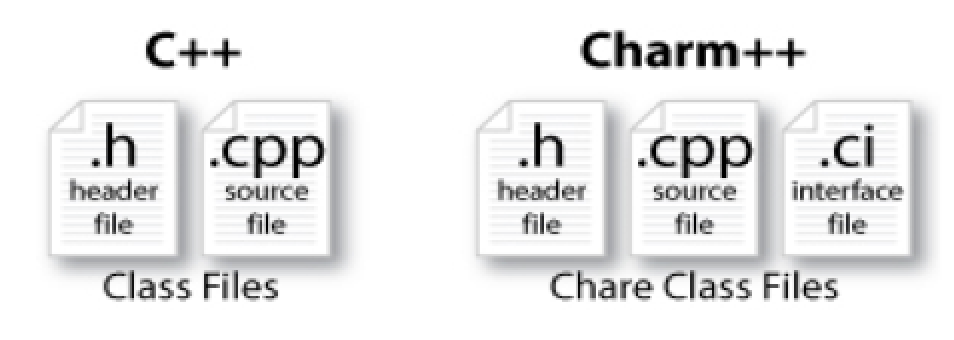
\includegraphics[width=0.6\textwidth]{charmFiles.png}
%   \end{center}
% \end{frame}

% \begin{frame}[fragile]
%   \frametitle{Charm Interface: Modules}
%   \begin{itemize}
%     \item Charm++ programs are organized as a collection of modules
%     \item Each module has one or more chares
%     \item The module that contains the \textit{mainchare}, is declared as the
%       \texttt{mainmodule}
%     \item Each module, when compiled, generates two files:
%       \code{<modulename>.decl.h} and \code{<modulename>.def.h}
%   \end{itemize}
%   \begin{center}
%   \begin{lstlisting}
%     [main]module <modulename> {
%       //... chare definitions ...
%     };
%   \end{lstlisting}
%   \end{center}
% \end{frame}

% \begin{frame}[fragile]
%   \frametitle{Charm Interface: Chares}
%   \begin{itemize}
%     \item Chares are parallel objects that are managed by the RTS
%     \item Each chare has a set \textit{entry methods}, which are asynchronous
%       methods that may be invoked remotely
%     \item The following code, when compiled, generates a C++ class
%       \code{CBase\_<charename>} that encapsulates the RTS object
%     \item This generated class is extended and implemented in the \texttt{.cpp}
%       file
%   \end{itemize}
%   \begin{lstlisting}
%     [main]chare <charename> {
%       //... entry method definitions ...
%     };

%     class MyChare : public CBase_<charename> {
%       //... entry method implementations ...
%     };
%   \end{lstlisting}
% \end{frame}

% \begin{frame}[fragile]
%   \frametitle{Charm Interface: Entry Methods}
%   \begin{itemize}
%   \item Entry methods are C++ methods that can be remotely and asynchronously
%     invoked by another chare
%   \end{itemize}
%   \begin{lstlisting}
%     entry <charename>(); /* constructor entry method */
%     entry void foo();
%     entry void bar(int param);

%     <charename>::<charename>() { /*... constructor code ...*/ }

%     <charename>::foo() { /*... code to execute ...*/ }

%     <charename>::bar(int param) { /*... code to execute ...*/ }
%   \end{lstlisting}
% \end{frame}

% \begin{frame}[fragile]
%    \frametitle{Charm Interface: \texttt{mainchare}}
%    \begin{itemize}
%      \item Execution begins with the \texttt{mainchare}'s constructor
%      \item The \texttt{mainchare}'s constructor takes a pointer to
%        system-defined class \code{CkArgMsg}
%      \item \code{CkArgMsg} contains \code{argv} and \code{argc}
%      \item The \texttt{mainchare} will often construct other parallel objects
%        and then wait for them to finish
%    \end{itemize}
% \end{frame}

% \begin{frame}[fragile]
%    \frametitle{Charm Termination}
%    \begin{itemize}
%    \item There is a special system call \code{CkExit()} that terminates the
%      parallel execution on all processors (but it is called on one processor)
%      and performs the requisite cleanup
%    \item The traditional \code{exit()} is insufficient because it only
%      terminates one process, not the entire parallel job (and will cause a
%      hang)
%    \item \code{CkExit()} should be called when you can safely terminate the
%      application (you may want to synchronize before calling this)
%    \end{itemize}
% \end{frame}

% \begin{frame}
%    \frametitle{Compiling a Charm++ Program}
%    \begin{center}
%      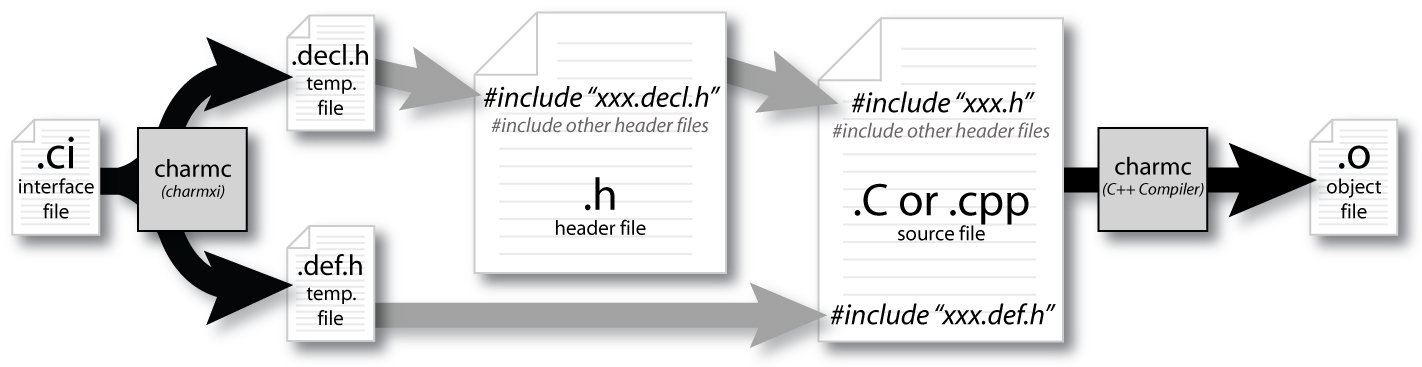
\includegraphics[width=0.9\textwidth]{charmCompile.jpg}
%    \end{center}
% \end{frame}

% \begin{frame}[fragile]
%    \frametitle{Hello World Example}\scriptsize
% \begin{itemize}
% \item \texttt{hello.ci} file
%    \begin{lstlisting}
% mainmodule hello {
%   mainchare Main {
%     entry Main(CkArgMsg *m);
%   };
% };
%    \end{lstlisting}
% \item \texttt{hello.cpp} file
% \lstset{basicstyle=\footnotesize}
%    \begin{lstlisting}
% #include <stdio.h>
% #include "hello.decl.h"

% struct Main : public CBase_Main {
%   Main(CkArgMsg* m) {
%     ckout << "Hello World!" << endl;
%     CkExit();
%   };
% };

% #include "hello.def.h"
%    \end{lstlisting}
% \end{itemize}
% \end{frame}

% \begin{frame}
%   \frametitle{Hello World Example}
%   \begin{itemize}
%     \item Compiling
%       \begin{itemize}
%       \item \texttt{charmc hello.ci}
%       \item \texttt{charmc -c hello.cpp}
%       \item \texttt{charmc -o hello hello.cpp}
%       \end{itemize}
%     \item Running
%       \begin{itemize}
%       \item \texttt{./charmrun +p7 ./hello}
%       \item The \texttt{+p7} tells the system to use seven cores
%       \end{itemize}
%     \end{itemize}
% \end{frame}

% \begin{frame}[fragile]
%   \frametitle{Creating a Chare}
%   \begin{itemize}
%     \item A chare declared as \code{chare <charename> \{...\};} can be
%       instantiated by the following call:
%   \end{itemize}
% \begin{lstlisting}
% CProxy_<charename>::ckNew(... constructor arguments ...);
% \end{lstlisting}
%   \begin{itemize}
%   \item To communicate with this class in the future, a \textit{proxy} to it
%     must be retained
%   \end{itemize}
% \begin{lstlisting}
% CProxy_<charename> proxy = 
%   CProxy_<charename>::ckNew(... constructor arguments ...);
% \end{lstlisting}
% \end{frame}

% \begin{frame}[fragile]
%   \frametitle{Chare Creation Example: \texttt{.ci} file}
%   \lstinputlisting{chareCreate.ci}
% \end{frame}

% \begin{frame}[fragile]
%   \frametitle{Chare Creation Example: \texttt{.cpp} file}
%   \lstinputlisting[basicstyle=\footnotesize]{chareCreate.C}
% \end{frame}

% \begin{frame}[fragile]
%   \frametitle{Asynchronous Methods}
%   \begin{itemize}
%   \item Entry methods are invoked by performing a C++ method call on a chare's
%     proxy
%   \end{itemize}
%   \begin{lstlisting}
% CProxy_<charename> proxy =
%   CProxy_<charename>::ckNew(... constructor arguments ...);

% proxy.foo();
% proxy.bar(5);
% \end{lstlisting}
% \begin{itemize}
% \item The \code{foo} and \code{bar} methods will then be executed with the
%   arguments, wherever \texttt{<charename>} happens to live
% \item The policy is one-at-a-time scheduling (that is, one entry method on one
%   chare executes on a processor at a time)
% \end{itemize}
% \end{frame}

% \begin{frame}[fragile]
%   \frametitle{Asynchronous Methods}
%   \begin{itemize}
%   \item Method invocation is not ordered (between chares, entry methods on one
%     chare, etc.)!
%   \item For example, if a chare executes this code:
%   \begin{lstlisting}
% CProxy_<charename> proxy = CProxy_<charename>::ckNew();
% proxy.foo();
% proxy.bar(5);
%   \end{lstlisting}
%   \item These prints may occur in \textbf{any} order
%   \begin{lstlisting}
% <charename>::foo() {
%   ckout << "foo executes" << endl;
% }

% <charename>::bar(int param) {
%   ckout << "bar executes with " << param << endl;
% }
% \end{lstlisting}
%   \end{itemize}
% \end{frame}

% \begin{frame}[fragile]
%   \frametitle{Asynchronous Methods}
%   \begin{itemize}
%   \item For example, if a chare invokes the same entry method twice:
%   \begin{lstlisting}
% proxy.bar(7);
% proxy.bar(5);
%   \end{lstlisting}%
%   \item These may be delivered in \textbf{any} order
%   \begin{lstlisting}
% <charename>::bar(int param) {
%   ckout << "bar executes with " << param << endl;
% }
% \end{lstlisting}
%   \item Output
% \begin{lstlisting}
% bar executes with 5
% bar executes with 7
% \end{lstlisting}
% \textbf{OR}
% \begin{lstlisting}
% bar executes with 7
% bar executes with 5
% \end{lstlisting}
%   \end{itemize}
% \end{frame}


% \begin{frame}[fragile]
%   \frametitle{Asynchronous Example: \texttt{.ci} file}
% \begin{lstlisting}
% mainmodule MyModule {
%   mainchare Main {
%     entry Main(CkArgMsg *m);
%   };
%   chare Simple {
%     entry Simple(double y);
%     entry void findArea(int radius, bool done);
%   };
% };
% \end{lstlisting}
% \end{frame}

% \begin{frame}[fragile]
%   \frametitle{Asynchronous Example: \texttt{.cpp} file}
% \begin{itemize}
%   \item Does this program execute correctly?
% \end{itemize}
% \scriptsize
% \begin{lstlisting}[basicstyle=\tiny]
% struct Main : public CBase_Main {
%   Main(CkArgMsg* m) {
%     double pi = 3.1415;
%     CProxy_Simple sim =  CProxy_Simple::ckNew(pi);
%     for (int i = 1; i< 10; i++) sim.findArea(i, false);
%     sim.findArea(10, true);
%   };
% };

% struct Simple : public CBase_Simple {
%  float y;
%  Simple(double pi) {
%    y = pi;
%    ckout << "Hello from a simple chare running on " << CkMyPe() << endl;
%  }
%  void findArea(int r, bool done) {
%    ckout << "Area of a circle of radius" << r << " is " << y*r*r << endl;
%    if (done) CkExit();
%  }
% };
% \end{lstlisting}
% \end{frame}

% \begin{frame}[fragile]
%   \frametitle{Data types and entry methods}
% \begin{itemize}
%   \item You can pass basic C++ types to entry methods (\texttt{int},
%     \texttt{char}, \texttt{bool}, etc.)
%   \item C++ STL data structures can be passed by including \texttt{pup\_stl.h}
%   \item Arrays of basic data types can also be passed like this:\\
% \begin{lstlisting}
% entry void foobar(int length, int data[length]);

% <charename>::foobar(int length, int* data) {
%  // ... foobar code ...
% }
% \end{lstlisting}
% \end{itemize}
% \end{frame}

% \begin{frame}[fragile]
%   \frametitle{Chare Proxies}
%   \begin{itemize}
%   \item A chare's own proxy can be obtained through a special variable
%     \code{thisProxy}
%   \item Chare proxies can also be passed so chares can learn about others
%   \item In this snippet, \code{<charename>} learns about a chare instance
%     \code{main}, and then invokes a method on it:
%   \end{itemize}
% \begin{lstlisting}
% entry void foobar2(CProxy_Main main);

% <charename>::foobar2(CProxy_Main main) {
%   main.foo();
% }
% \end{lstlisting}
% \end{frame}

% \begin{frame}[fragile]
%   \frametitle{Chare Proxy Example}
% \texttt{.ci} file
% \begin{lstlisting}[basicstyle=\tiny]
%   mainchare Main {
%     entry Main(CkArgMsg *m);
%     entry void finished();
%   };
%   chare Simple {
%     entry Simple(CProxy_Main mainProxy);
%   };
% \end{lstlisting}
% \texttt{.cpp} file
% \begin{lstlisting}[basicstyle=\tiny]
%   struct Main : public CBase_Main {
%     Main(CkArgMsg *m) {
%       CProxy_Simple::ckNew(thisProxy);      
%     }
%     void finished() { CkExit(); }
%   };
%   struct Simple : public CBase_Simple {
%     Simple(CProxy_Main mainProxy) {
%       ckout << "Hello from Simple" << endl;
%       mainProxy.finished();
%     }
%   };
% \end{lstlisting}
% \end{frame}

% \begin{frame}[fragile]
%   \frametitle{Readonlys}
%   \begin{itemize}
%   \item A \textit{readonly} is a global (within a module) read-only variable
%     that can only be written to in the \texttt{mainchare}'s constructor
%   \item Can then be read (\textbf{not written!}) by any chare in the module
%   \item It is declared in the \texttt{.ci} file:
% \begin{lstlisting}
%   readonly <type> <name>;
%   readonly CProxy_Main mainProxy;
%   readonly int numChares;
% \end{lstlisting}
%   \item And defined the the \texttt{.cpp} file:
% \begin{lstlisting}
%   <type> <name>;
%   CProxy_Main mainProxy;
%   int numChares;
% \end{lstlisting}
%   \item And set in the \texttt{mainchare}'s constructor
% \begin{lstlisting}
%   <charename>::<charename>(CkArgMsg *m) {
%     mainProxy = thisProxy;
%     numChares = 10;
%   }
% \end{lstlisting}


%   \end{itemize}
% \end{frame}

% \begin{frame}[fragile]
%   \frametitle{PI Example}
%   \lstinputlisting{pi.ci}  
% \end{frame}

% \begin{frame}[fragile]
%   \frametitle{PI Example}
%   \lstinputlisting[basicstyle=\tiny]{piMaster.C}
% \end{frame}

% \begin{frame}[fragile]
%   \frametitle{PI Example}
%   \lstinputlisting{piWorker.C}
% \end{frame}

\begin{frame}[fragile]
  \frametitle{Task Parallelism}
  \begin{itemize}
    \item Divide-and-conquer
      \begin{itemize}
      \item Each \textit{task} recursively creates $n$ tasks that divide the
        problem into subproblems
      \item Each task $t$ then waits for all $n$ tasks to finish and then may
        `combine' the responses
      \item At some point the recursion stops (at the bottom of the tree), and
        some sequential kernel is executed
      \item Then the result is propagated upward in the tree recursively
      \item Examples: fibonacci, quick sort, $\ldots$
      \end{itemize}
  \end{itemize}
\end{frame}


\begin{frame}[fragile]
  \frametitle{Task Parallelism}
  \begin{itemize}
    \item State-space search
      \begin{itemize}
      \item Each \textit{task} recursively creates $n$ tasks to partition the
        search space
      \item If the problem is one-solution search, as soon as a task encounters
        a solution, the program may need to terminate
        \begin{itemize}
          \item Kill-chasing problem
        \end{itemize}
      \end{itemize}
      \item All-solution search may require behaviour much like
        divide-and-conquer where values are combined
        \begin{itemize}
        \item Example: all-solution nqueens
        \item Number of solutions are accumulated recursively up the tree
        \end{itemize}
  \end{itemize}
\end{frame}

\begin{frame}[fragile]
  \frametitle{Fibonacci Example}
  \begin{itemize}
    \item Each \code{Fib} chare is a task that performs one of two actions:
      \begin{itemize}
        \item Creates two new \code{Fib} chares to compute $fib(n-1)$ and
          $fib(n-2)$ and then waits for the response, adding up the two
          responses when they arrive
          \begin{itemize}
          \item After both arrive, sends a response message with the result to
            the parent task
          \item Or prints the value and calls \code{CkExit()} if it is the root
          \end{itemize}
        \item If $n = 1$ or $n = 0$ (passed down from the parent) it sends a
          response message with $n$ back to the parent task
      \end{itemize}
  \end{itemize}
\end{frame}

\begin{frame}[fragile]
  \frametitle{Fibonacci Example}
  \lstinputlisting{fib1.ci}
\end{frame}

\begin{frame}[fragile]
  \frametitle{Fibonacci Example}
  \lstinputlisting[basicstyle=\tiny]{fib1.C}
\end{frame}

\begin{frame}[fragile]
  \frametitle{Fibonacci Execution}
   \begin{center}
     \includegraphics<1>[width=0.9\textwidth]{diagrams/tree1.pdf}
     \includegraphics<2>[width=0.9\textwidth]{diagrams/tree2.pdf}
     \includegraphics<3>[width=0.9\textwidth]{diagrams/tree3.pdf}
     \includegraphics<4>[width=0.9\textwidth]{diagrams/tree4.pdf}
     \includegraphics<5>[width=0.9\textwidth]{diagrams/tree5.pdf}
     \includegraphics<6>[width=0.9\textwidth]{diagrams/tree6.pdf}
     \includegraphics<7>[width=0.9\textwidth]{diagrams/tree7.pdf}
     \includegraphics<8>[width=0.9\textwidth]{diagrams/tree8.pdf}
     \includegraphics<9>[width=0.9\textwidth]{diagrams/tree9.pdf}
     \includegraphics<10>[width=0.9\textwidth]{diagrams/tree10.pdf}
   \end{center}
\end{frame}

\begin{frame}[fragile]
  \frametitle{Fibonacci Performance}
  \begin{itemize}
  \item How much work/computation does each chare do in this example?
  \item What are some of the overheads of this approach?
  \item Is there way we can reduce/amortize the overhead?
  \end{itemize}
\end{frame}

\begin{frame}[fragile]
  \frametitle{Possible Solution}
  \begin{itemize}
  \item Set a sequential threshold in the computational tree
    \begin{itemize}
    \item Past this threshold (i.e. when $n < threshold$), instead of
      constructing two new chares, compute the fibonacci sequentially
    \end{itemize}
  \end{itemize}
  \begin{center} 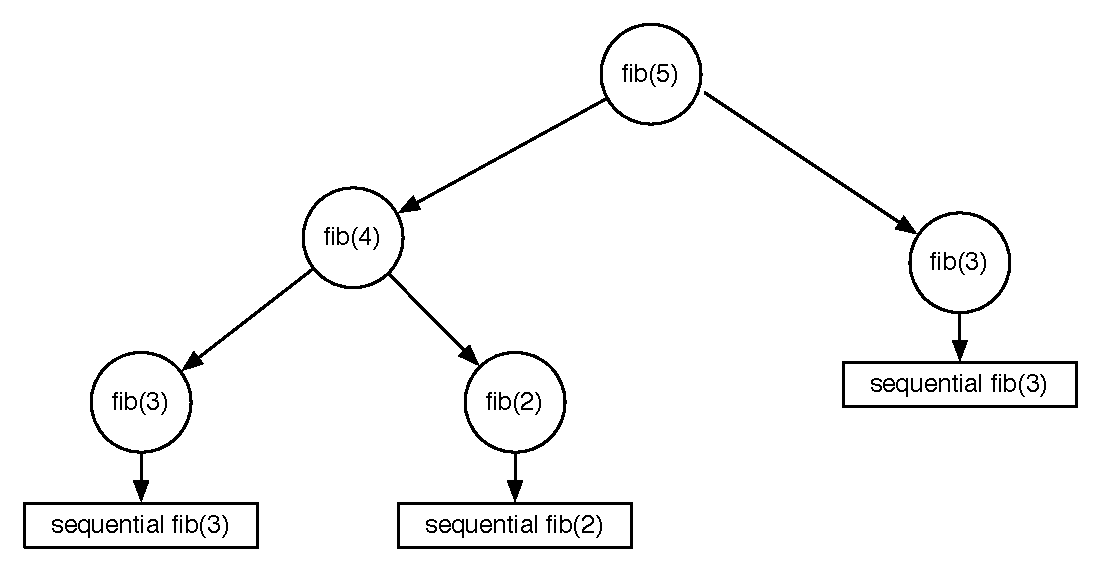
\includegraphics[width=0.7\textwidth]{diagrams/tree-threshold.pdf} \end{center}
  \begin{itemize}
    \item $fib(5), fib(4)$ are fine grains, $fib(3), fib(2)$ are coarser grains
    \item The coarser grains now amortize the cost of the fine-grained execution
  \end{itemize}
\end{frame}

\begin{frame}[fragile]
  \frametitle{Fibonacci w/Threshold Example}
  \lstinputlisting[basicstyle=\tiny]{fib2.C}
\end{frame}

\begin{frame}
  \frametitle{Amdahls’s Law and Grainsize}
  \begin{itemize}
    \item Original ``law'':
      \begin{itemize}
      \item If a program has $K$\% sequential section, then speedup is limited
        to $\frac{100}{K}$.
        \begin{itemize}
        \item If the rest of the program is parallelized completely
        \end{itemize}
      \end{itemize}
    \item Grainsize corollary:
      \begin{itemize}
      \item If any individual piece of work is $> K$ time units, and the
        sequential program takes $T_{seq}$, 
        \begin{itemize}
        \item Speedup is limited to $\frac{T_{seq}}{K}$
        \end{itemize}
      \end{itemize}
    \item So:
      \begin{itemize}
      \item Examine performance data via histograms to find the sizes of
        remappable work units
      \item If some are too big, change the decomposition method to make
        smaller units
      \end{itemize}
  \end{itemize}
\end{frame}

\begin{frame}
  \frametitle{Grainsize}
  \begin{itemize}
    \item (working) Definition: the amount of computation per potentially
      parallel event (task creation, enqueue/dequeue, messaging, locking. .)
  \end{itemize}
  \begin{center} 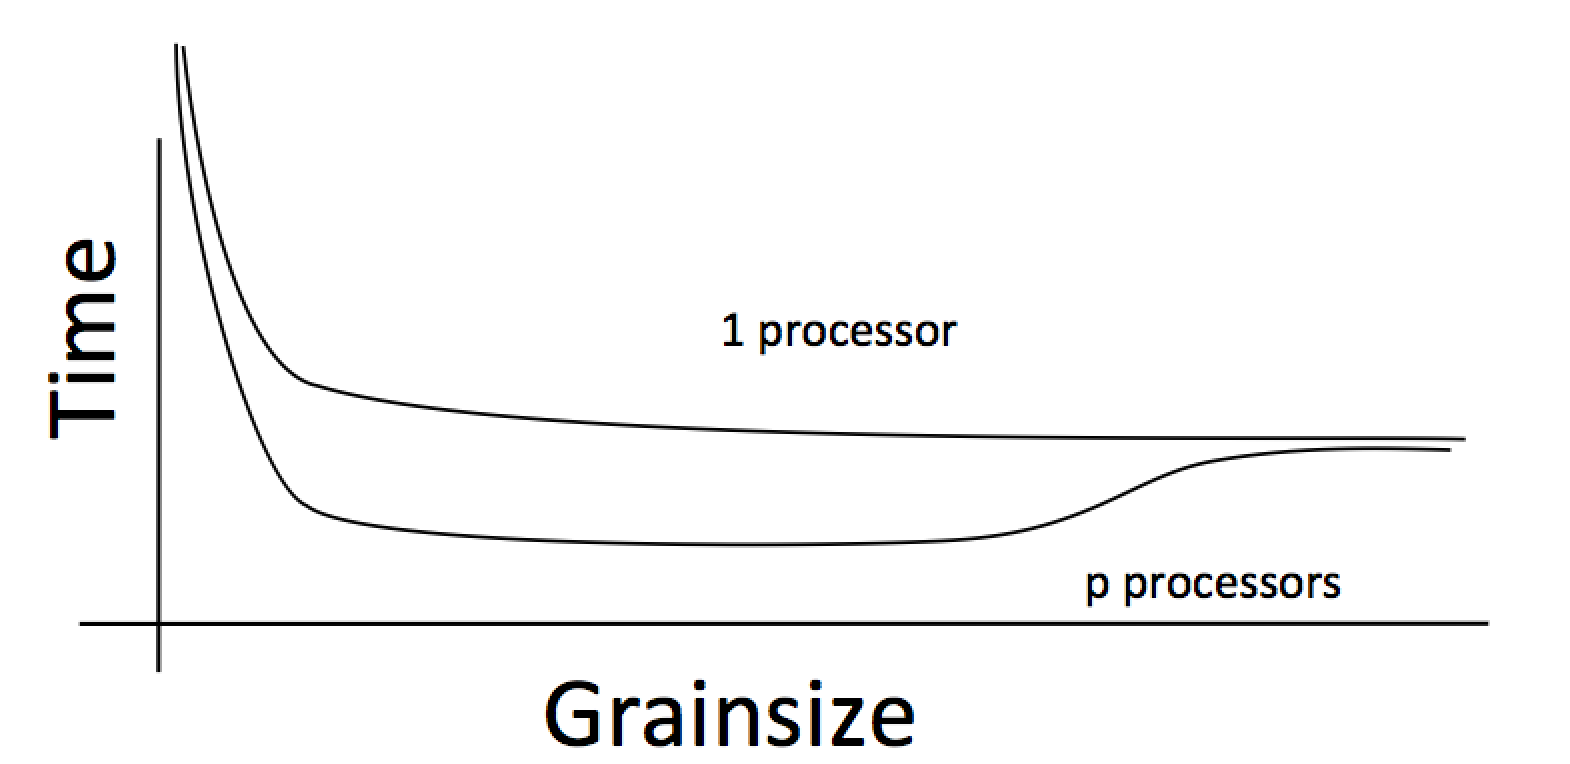
\includegraphics[width=0.7\textwidth]{grain1.png} \end{center}
\end{frame}

\begin{frame}
  \frametitle{Grainsize and Overhead}
  \begin{itemize}
    \item What is the ideal grainsize?
    \item Should it depend on the number of processors?
    
  \end{itemize}
  \begin{center}
    $T_1 = T \left( 1 + \frac{v}{g} \right)$\\
    $T_p = max \left\{ g, \frac{T_1}{p} \right\}$\\
    $T_p = max \left\{ g, \frac{T\left( 1+ \frac{v}{g} \right)}{p} \right\}$\\
    $v$: overhead per message,\\
    $T_p$: $p$ processor completion time\\
    $g$: grainsize (computation per message)
  \end{center}
\end{frame}

\begin{frame}
  \frametitle{Grainsize and Scalability}
  \begin{center} 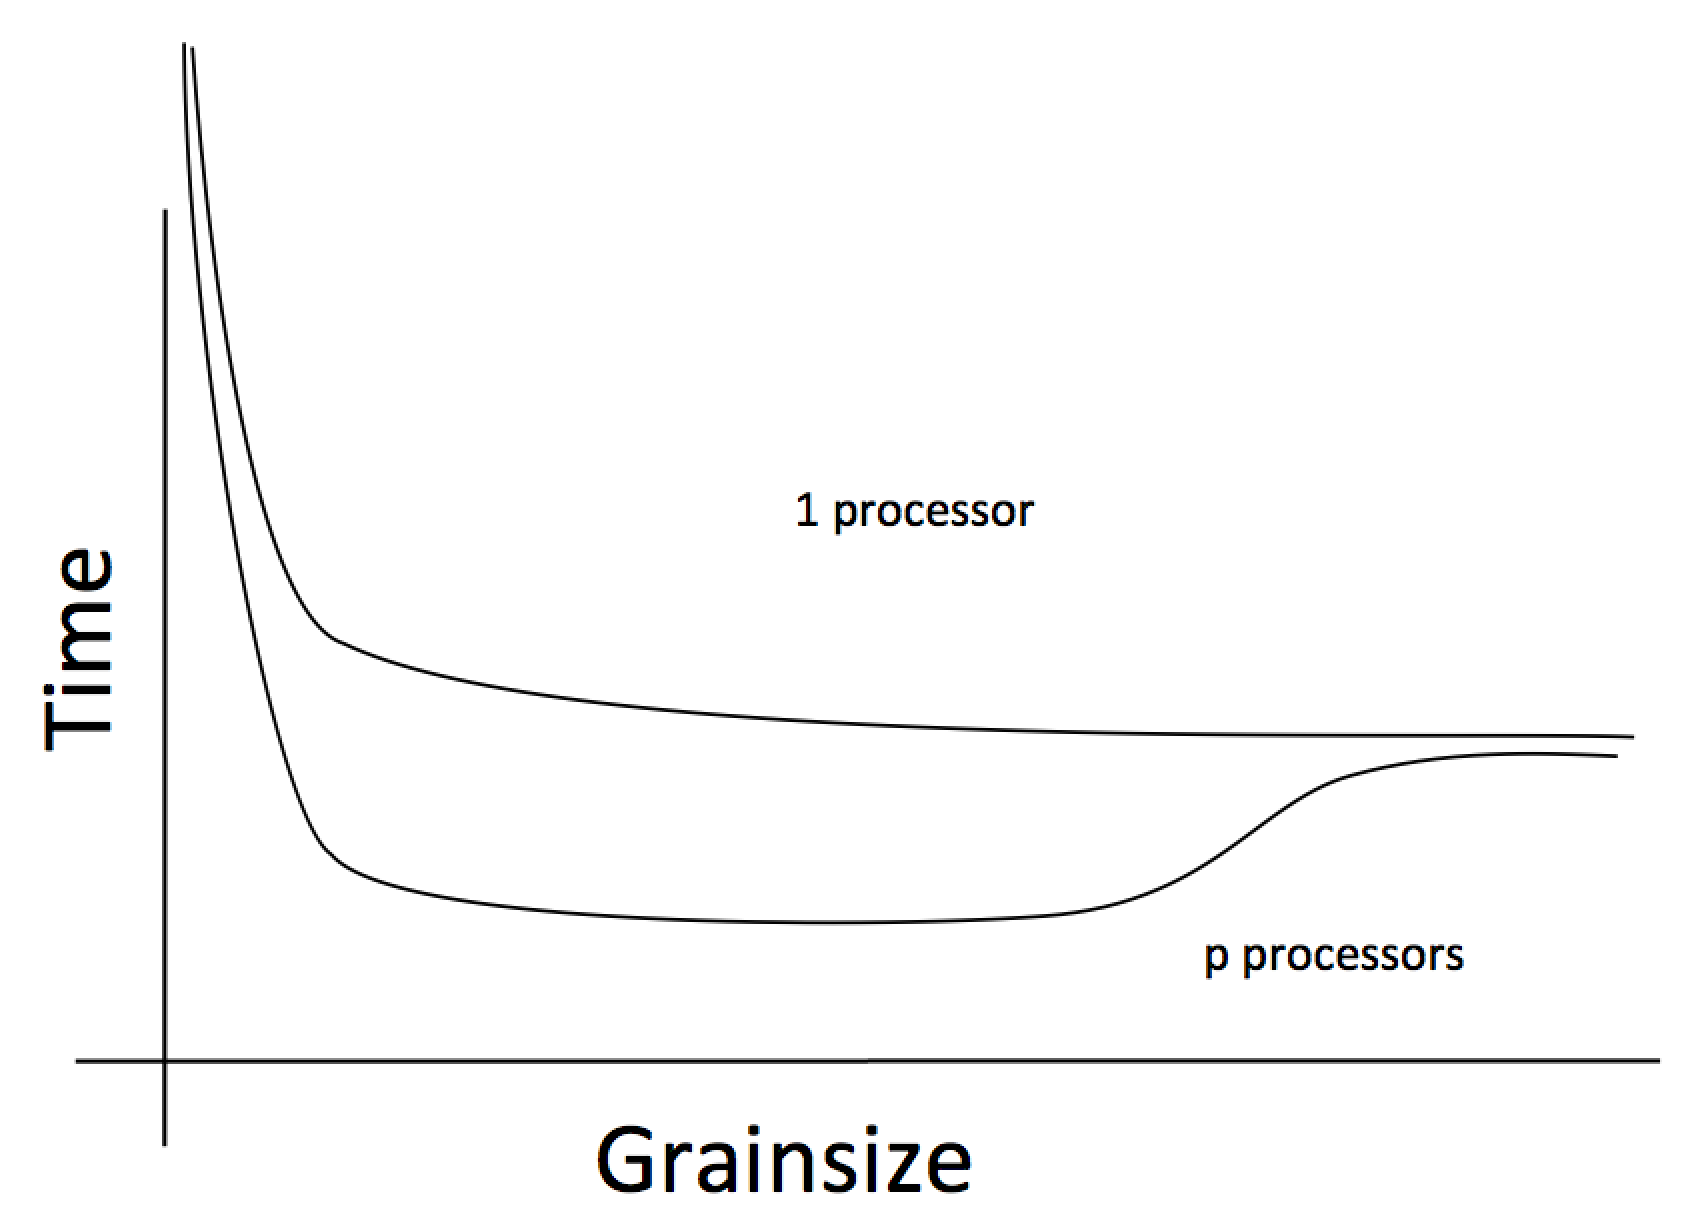
\includegraphics[width=0.7\textwidth]{grain2.png} \end{center}
\end{frame}

\begin{frame}
  \frametitle{Rules of thumb for grainsize}
  \begin{itemize}
    \item Make it as small as possible, as long as it amortizes the overhead
    \item More specifically, ensure:
      \begin{itemize}
      \item \textit{Average} grainsize is greater than $kv$ (say $10v$)
      \item No single grain should be allowed to be too large 
        \begin{itemize}
          \item Must be smaller than $\frac{T}{p}$, but actually we can express
            it as:
          \item Must be smaller than $kmv$ (say $100v$)
        \end{itemize}
      \end{itemize}
    \item Important corollary:
      \begin{itemize}
      \item You can be at close to optimal grainsize without having to think
        about $p$, the number of processors
      \end{itemize}
  \end{itemize}
\end{frame}

\begin{frame}
  \frametitle{How to determine/ensure grainsize}
  \begin{itemize}
    \item Compiler techniques can help, but only in some cases
      \begin{itemize}
        \item Note that they don't need precise determination of grainsize,
          just one that will satisfy a broad inequality
          \begin{itemize}
            \item $kv < g < mkv$ ($10v < g < 100v$)
          \end{itemize}
      \end{itemize}
  \end{itemize}
\end{frame}

\end{document}

